\documentclass{article}
\usepackage{graphicx}
\usepackage{amsmath}
\usepackage[utf8]{inputenc}
\usepackage{geometry}
 \geometry{
 a4paper,
 total={170mm,257mm},
 left=20mm,
 top=20mm,
 }
 
\begin{document}	
	\section{Ejercicio 4}
	\subsection{Introducción}
		\hspace{10mm} Para implementar un circuito que convierta un numero binario de 4 bits en su complemento a dos se empezó pensando este circuito como una caja negra con 4 entradas y 4 salidas:
		\begin{figure}[h!]
			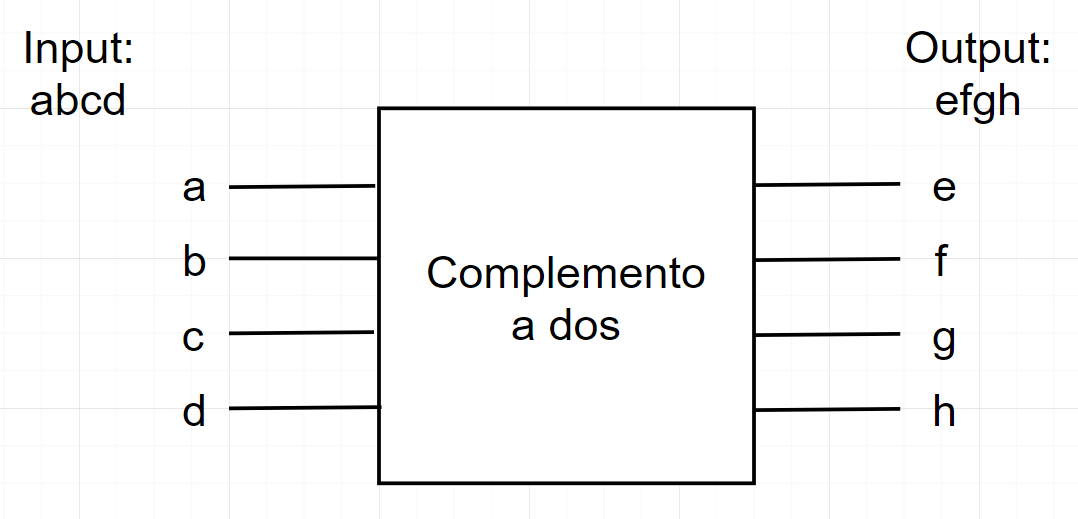
\includegraphics[width=\linewidth,scale=0.5]{comp2.png}
  			\caption{Caja Negra Complemento a 2}
		\end{figure}
		\newline \hspace{10mm} A su vez, sabemos que el complemento a dos se realiza aplicando el complemento a uno y luego sumando uno al resultado. Por lo que se puede representar mediante el siguiente conjunto de "cajas negras":
		\begin{figure}[h!]
			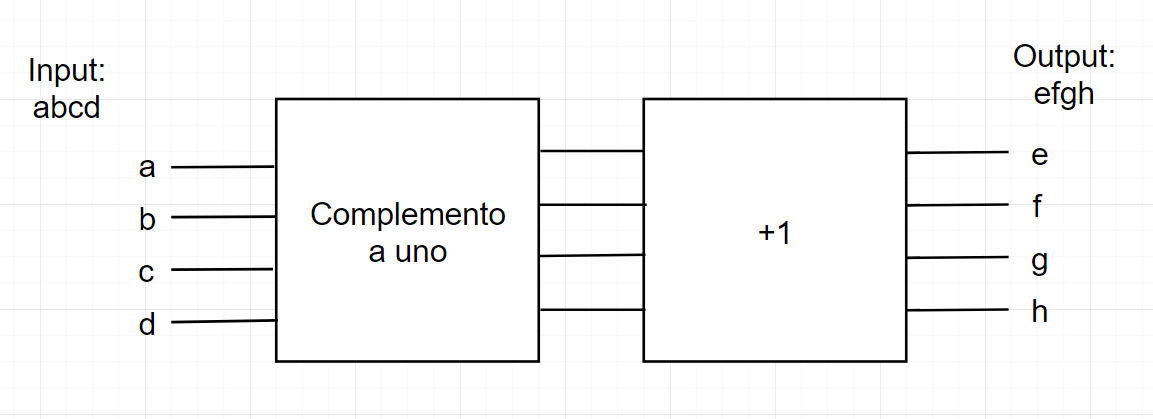
\includegraphics[width=\linewidth,scale=0.5]{comp1+1.png}
  			\caption{Caja Negra Complemento a 2}
		\end{figure}
		\newline \hspace{10mm} La salida tras el complemento a uno sabemos que es cada bit negado, es decir que atraviesan una compuerta NOT. De esta manera a la salida de el complemento a uno que se obtiene es: 
		\newline \centerline{$\overline{a} \overline{b} \overline{c} \overline{d}$} 
		\hspace{10mm} Ahora lo único que falta es sumarle uno.
	\subsection{Expresion de la salida en minterminos}
		\hspace{10mm} La expresión de la salida queda determinada por las entrada a través de la siguiente formula deducida en la introducción:
		\newline \centerline{$\overline{a} \overline{b} \overline{c} \overline{d}$}
		\newline \centerline{$+0001$}
		\newline \centerline{$----$}
		\newline \centerline{$efgh$}	
		\newline \hspace{10mm} Para la creación de las tablas de valor se debe observar que el output de cada bit depende de el resultado de el input de los bits menos significativos que con el que se esta trabajando.
		\newline Para el BMS la tabla de verdad es muy simple y no vale la pena el uso de minterminos por lo que se vera a continuación:
		\begin{table}[h!]
			\begin{center}
				\caption{Tabla para bit h}
				\begin{tabular}{l|c|r}
				\textbf{$\overline{d}$} & \textbf{1} & \textbf{h}\\
				\hline
				1 & 1 & 0 \\
				0 & 1 & 1 \\			
				\end{tabular}
			\end{center}
		\end{table}
		\newline Fácilmente de la tabla se puede observar que h resulta ser la entrada negada. Por lo que resulta la primera relación de entrada-salida:
		\begin{equation}
			\centerline{$h(d)=\overline{\overline{d}}$}
		\end{equation}
		\newline Para la salida correspondiente a el bit g la tabla de verdad es de la siguiente manera:
		\begin{table}[h!]
			\begin{center}
				\caption{Tabla para bit g}
				\begin{tabular}{l|c|r}
				\textbf{$\overline{c}$} & \textbf{$\overline{d}$} & \textbf{g}\\
				\hline
				0 & 0 & 0 \\
				0 & 1 & 1 ($m_{1}$) \\	
				1 & 0 & 1 ($m_{2}$)\\
				1 & 1 & 0 \\			
				\end{tabular}
			\end{center}
		\end{table}	
		\newline Al escribir la salida en función de los minterminos se llega a la siguiente expresión:
		\newline \centerline{$g(c,d)=m_{1}+m_{2}$}
		\begin{equation}
			\centerline{$g(c,d)=\overline{\overline{c}}\overline{d}+\overline{c}\overline{\overline{d}}$}
		\end{equation}
		\newline Ahora para el bit f se requiere una tabla de verdad de tres variables ya que ahora depende del carry causado por las variables de entrada c y d:
		\begin{table}[h!]
			\begin{center}
				\caption{Tabla para bit f}
				\begin{tabular}{l|c|c|r}
				\textbf{$\overline{b}$} & \textbf{$\overline{c}$} & \textbf{$\overline{d}$} & \textbf{f}\\
				\hline
				0 & 0 & 0 & 0\\
				0 & 0 & 1 & 0\\	
				0 & 1 & 0 & 0\\
				0 & 1 & 1 & 1($m_{3}$)\\
				1 & 0 & 0 & 1($m_{4}$)\\
				1 & 0 & 1 & 1($m_{5}$)\\	
				1 & 1 & 0 & 1($m_{6}$)\\
				1 & 1 & 1 & 0\\				
				\end{tabular}
			\end{center}
		\end{table}
		\newline Al escribir la salida en función de los minterminos se llega a la siguiente expresión:
		\newline \centerline{$f(b,c,d)=m_{3}+m_{4}+m_{5}+m_{6}$}
		\begin{equation}
			\centerline{$f(b,c,d)=\overline{\overline{b}}\overline{c}\overline{d}+\overline{b}\overline{\overline{c}}\overline{\overline{d}}+\overline{b}\overline{\overline{c}}\overline{d}+\overline{b}\overline{c}\overline{\overline{d}}$}
		\end{equation}
		\newline Para el bit e la tabla de verdad es la siguiente:
			\begin{table}[h!]
			\begin{center}
				\caption{Tabla para bit e}
				\begin{tabular}{l|c|c|c|r}
				\textbf{$\overline{a}$} & \textbf{$\overline{b}$} & \textbf{$\overline{c}$} & \textbf{$\overline{d}$} & \textbf{e}\\
				\hline
				0 & 0 & 0 & 0 & 0\\
				0 & 0 & 0 & 1 & 0\\	
				0 & 0 & 1 & 0 & 0\\
				0 & 0 & 1 & 1 & 0\\
				0 & 1 & 0 & 0 & 0\\
				0 & 1 & 0 & 1 & 0\\	
				0 & 1 & 1 & 0 & 1($m_{6}$)\\
				0 & 1 & 1 & 1 & 1($m_{7}$)\\		
				1 & 0 & 0 & 0 & 1($m_{8}$)\\
				1 & 0 & 0 & 1 & 1($m_{9}$)\\	
				1 & 0 & 1 & 0 & 1($m_{10}$)\\
				1 & 0 & 1 & 1 & 1($m_{11}$)\\
				1 & 1 & 0 & 0 & 1($m_{12}$)\\
				1 & 1 & 0 & 1 & 1($m_{13}$)\\	
				1 & 1 & 1 & 0 & 1($m_{14}$)\\
				1 & 1 & 1 & 1 & 0\\			
				\end{tabular}
			\end{center}
		\end{table}
		\newline Al escribir la salida en función de los minterminos se llega a la siguiente expresión:
		\newline \centerline{$e(a,b,c,d)=m_{6}+m_{7}+m_{8}+m_{9}+m_{10}+m_{11}+m_{12}+m_{13}+m_{14}$}
		\begin{equation}
			\centerline{$e(a,b,c,d)=\overline{\overline{a}}\overline{b}\overline{c}\overline{d}+\overline{a}\overline{\overline{b}}\overline{\overline{c}}\overline{\overline{d}}+\overline{a}\overline{\overline{b}}\overline{\overline{c}}\overline{d}+\overline{a}\overline{\overline{b}}\overline{c}\overline{\overline{d}}+\overline{a}\overline{\overline{b}}\overline{c}\overline{d}+\overline{a}\overline{b}\overline{\overline{c}}\overline{\overline{d}}+\overline{a}\overline{b}\overline{\overline{c}}\overline{d}+\overline{a}\overline{b}\overline{c}\overline{\overline{d}}$}
		\end{equation}
	\subsection{Simplificación de las ecuaciones resultantes}
		\hspace{10mm} Para reducir las 4 expresiones resultantes procedemos a utilizar la propiedad:
		\newline \centerline{$\overline{\overline{a}}=a$}
		Lo cual da como resultado las 4 siguientes ecuaciones:
			\begin{align*}
				h & = d\\
				g & = c\overline{d}+\overline{c}d\\
				f & = b\overline{c}\overline{d}+\overline{b}cd+\overline{b}c\overline{d}+\overline{b}\overline{c}d\\
				e & = a\overline{b}\overline{c}\overline{d}+\overline{a}bcd+\overline{a}bc\overline{d}+\overline{a}b\overline{c}d+\overline{a}b\overline{c}\overline{d}+\overline{a}\overline{b}cd+\overline{a}\overline{b}c\overline{d}+\overline{a}\overline{b}\overline{c}d
			\end{align*}
			De estas cuatro expresiones las primeras no son posibles de reducir mas. Pero la tercera y cuarta son posibles de reducir con el uso de las siguientes propiedades:
			\begin{align*}
				a+a & = a\\
				a+\overline{a} & = 1\\
				ab+cb & = b(a+c)
			\end{align*} 
			La primera propiedad significa que puedo sumar uno de los minterminos a la expresión que esta no se vera afectada si ese mintermino ya pertenecía a la expresión. Con la segunda expresión puedo sacar 'factor común' los términos que difieran en una variable y su complemento de manera que al hacer el factor común quede de la forma $f(a,b,...)(z+\overline{z})$ y así utilizar la tercera propiedad que simplifica esa expresión a $f(a,b,...)$. De esta manera las ecuaciones se simplifican a su forma final que es de la siguiente manera:
			\begin{align*}
				h & = d\\
				g & = c\overline{d}+\overline{c}d\\
				f & = b\overline{c}\overline{d}+\overline{b}c+\overline{b}d\\
				e & = a\overline{b}\overline{c}\overline{d}+\overline{a}\overline{c}d+\overline{a}\overline{b}c+\overline{a}b
			\end{align*}
	\subsection{Circuito Resultante}
	Al implementar las expresiones halladas en la sección anterior con compuertas AND, OR y NOT se llega al siguiente circuito: 
	\begin{figure}[h!]
			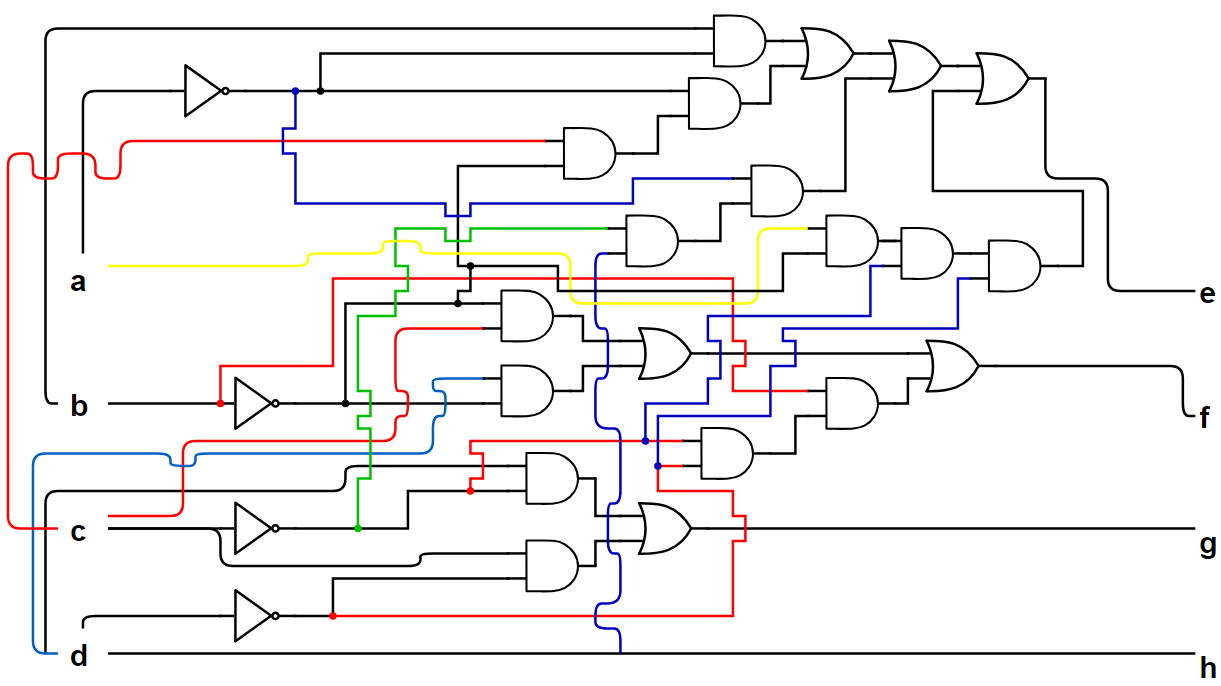
\includegraphics[width=\linewidth,scale=0.5]{circuitoEj4.png}
  			\caption{Circuito de conversión a complemento a dos}
		\end{figure}
\end{document}
